\chapter{Introduction}
In satellite applications, radio communication is the most important method for controlling the satellite state and issuing any commands to it.
COŚ TUTAJ WIECEJ TYLKO NIE MAM POJĘCIA CO


\section{Scope of the thesis}
The aim of this thesis was to design, verify, validate and deploy the communication system for second Polish satellite, PW-Sat2. The design covers all aspects of communication link design from the system point of view: the link design, space and ground segments and testing all the subsystems. Thesis should describe the choices and the practical design of the low-cost satellite link using both off-the-shelf hardware, custom designed components and Software Defined Radio, with custom digital signal processing. The designed system should provide a two-way data link between the operator and the satellite. Finally, the system was tested on the orbit, proving its parameters and reliability.

\section{PW-Sat2}
The presented system was design specifically to be deployed on-board the PW-Sat2 satellite.  The main aim of PW-Sat2 is to test out a new and innovative deorbit technology. PW-Sat2 was launched on Low Earth Orbit or 3rd of December 2018 on-board SpaceX Falon 9 rocket. PW-Sat2 was placed on a sun-synchronous, polar, circular, \SI{590}{\kilo\meter}-orbit.
In the figure \ref{PW-Sat_render_01} an exploded render of PW-Sat2 is presented.
\begin{figure}
    \centering
    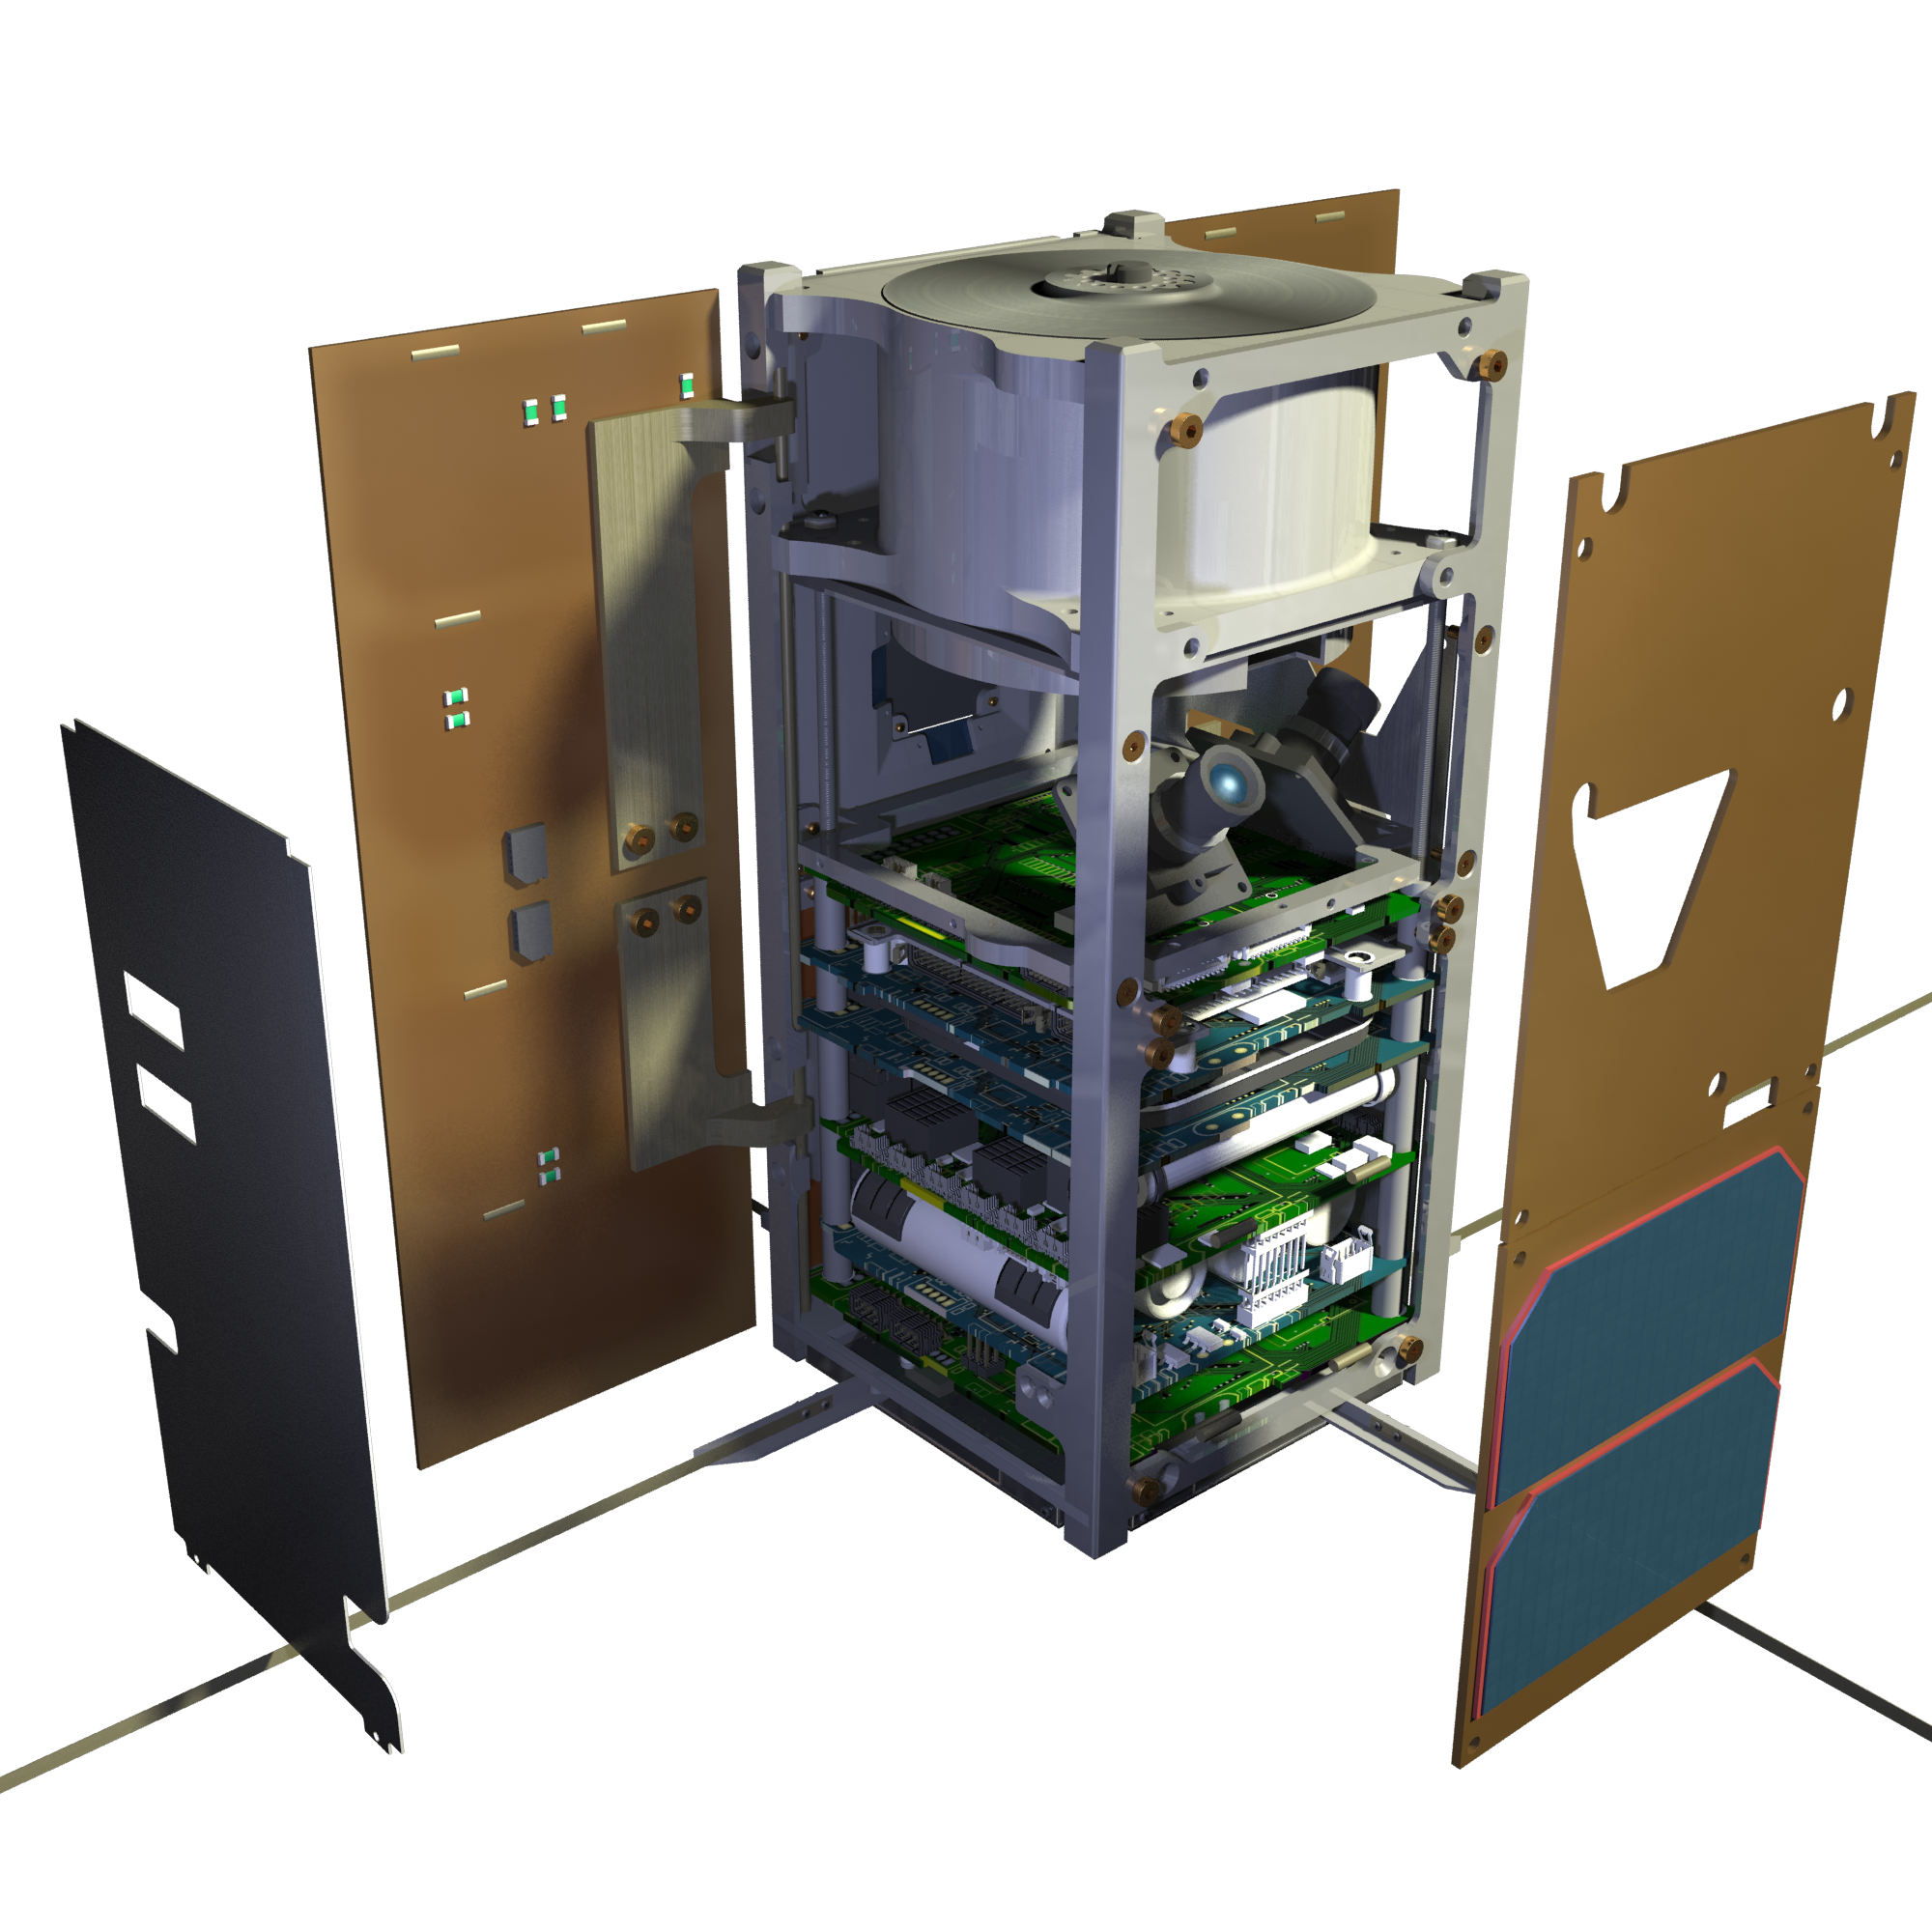
\includegraphics[width=0.65\paperwidth]{img/1/PW-Sat2_render_01.png}
    \caption{PW-Sat2 render. Source: \cite{PW_sat2_photo}}
    \label{PW-Sat_render_01}
\end{figure}


\subsection{Primary mission}
The primary mission of PW-Sat2 is to test the innovative deorbit technology - the deorbit sail. After satellite operations phase end, the deorbit sail will open and increase the atmospheric drag, shortening the life time. A render of PW-Sat2 with opened sail is shown in the figure \ref{PW-Sat_render_sail}. As seen in the figure, the deorbit sail material is stretched on four flat springs, made of metal. The material of the sail is the \SI{5}{\micro\meter} mylar foil covered with aluminum. The sail is placed very close to the antennas - therefore it can influence the antenna pattern and matching. 
\begin{figure}
    \centering
    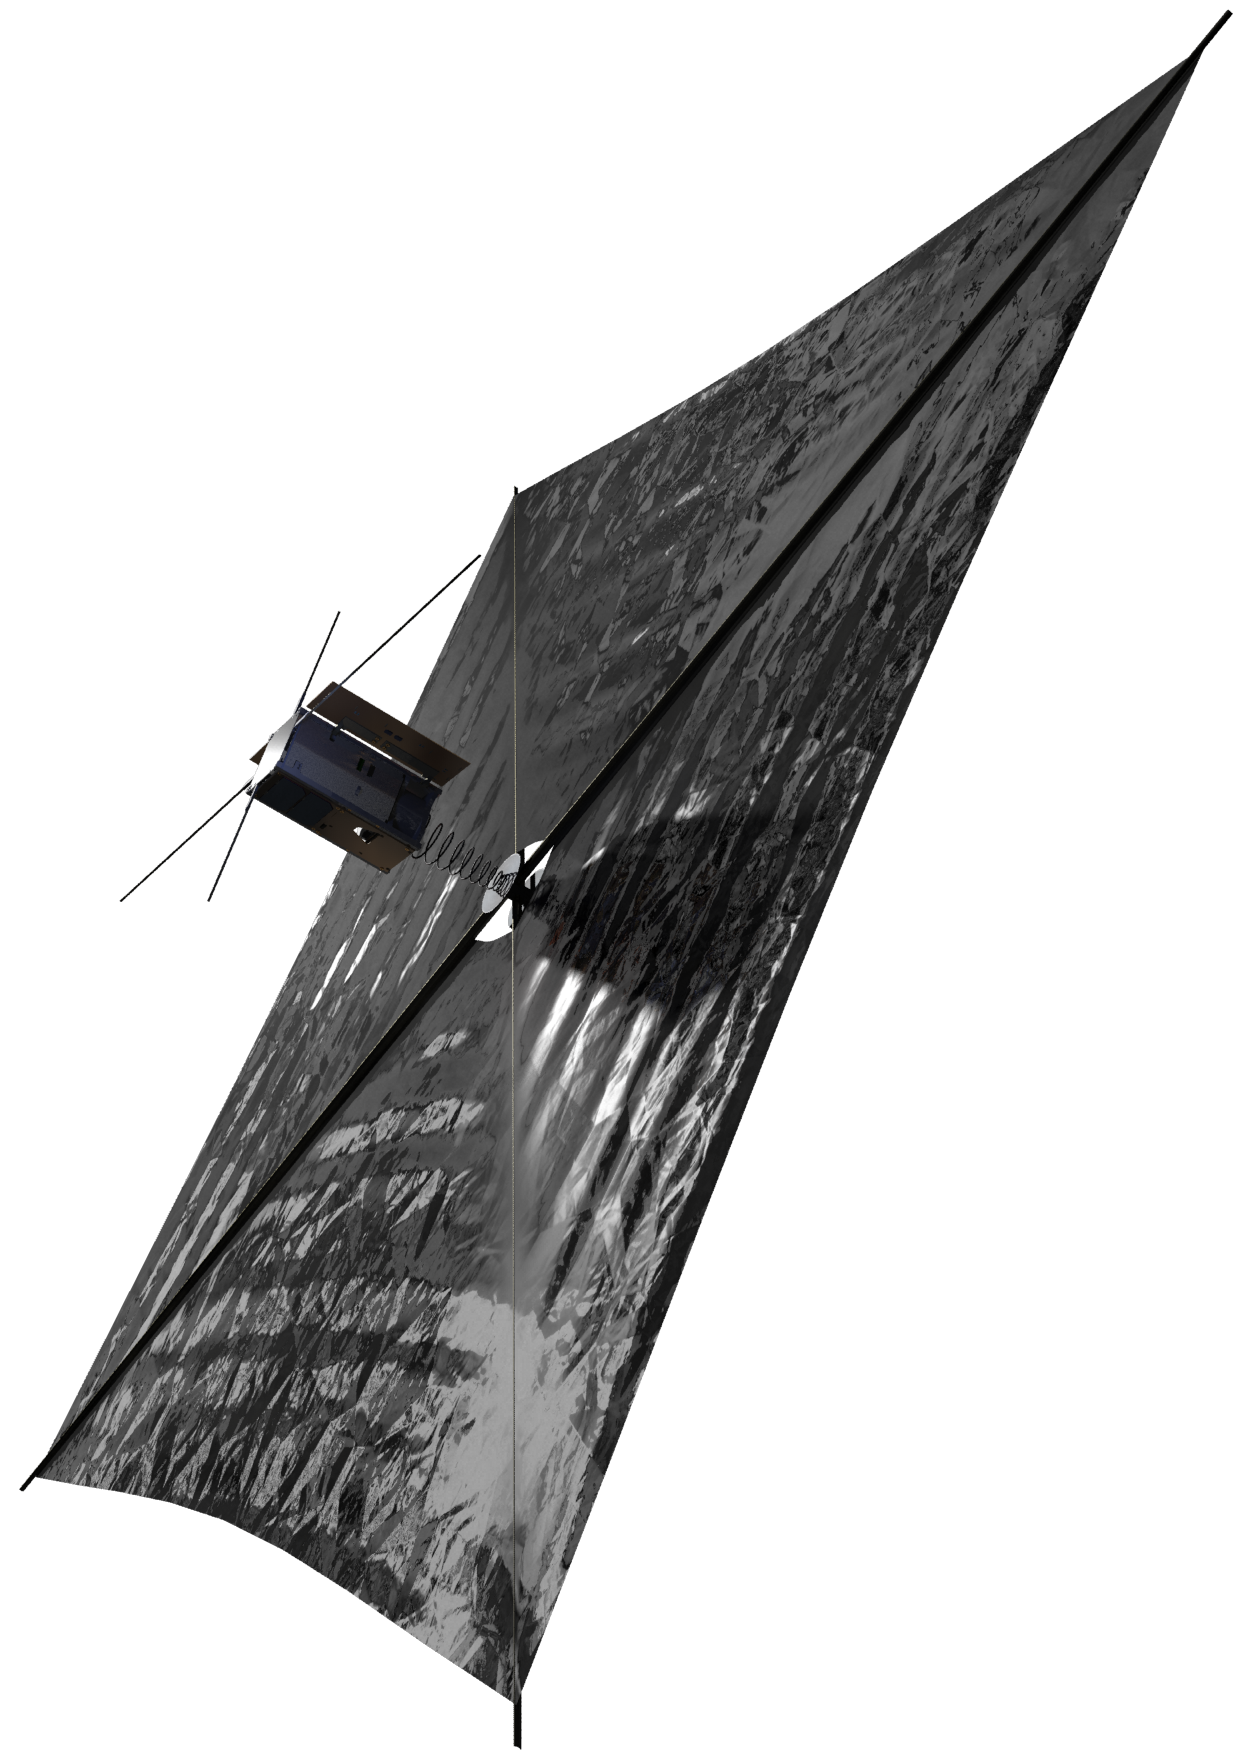
\includegraphics[width=0.38\paperwidth]{img/1/PW-Sat2_render_02.png}
    \caption{PW-Sat2 with opened sail and antennas. Source: \cite{PW_sat2_photo}}
    \label{PW-Sat_render_sail}
\end{figure}


\subsection{Secondary mission goals}
PW-Sat2 have also three secondary experiments, executed by the command from the operators on the ground. Those experiments will be ran according when the link and power budget will allow to. Secondary experiments include:
\begin{itemize}
    \item RadFET - ionising radiation sensor, which will measure threshold voltages on P-MOS transistors to estimate the TID absorbed by the satellite.
    \item Sun Sensor -  it will provide an orientation data which will be compared with the commercial system readings. During the experiment, \si{12} Ambient Light Sensors will provide information about their illumination, allowing the software to calculate angles to the Sun.
    \item Cameras - two VGA-resolution (\si{640}x\si{480}~px) on-board cameras with small and non-complicated optics which will allow to observe some parts of the deorbitation sail during its opening, monitor the sail condition during deorbitation phase and to take photos of the Earth.
\end{itemize}


\subsection{Solar array deployment}
PW-Sat2 have two solar panels which are deployed by the command from the On-Board Computer on the request of the satellite operator from the ground. Solar panels are mounted on two opposite directions, open and create one large panel as seen on the figure \ref{PW-Sat_solar_panels}. The wings, on which solar panels are mounted, are made from aluminum, therefore their deployment can change the antennas parameters.
\begin{figure}
    \centering
    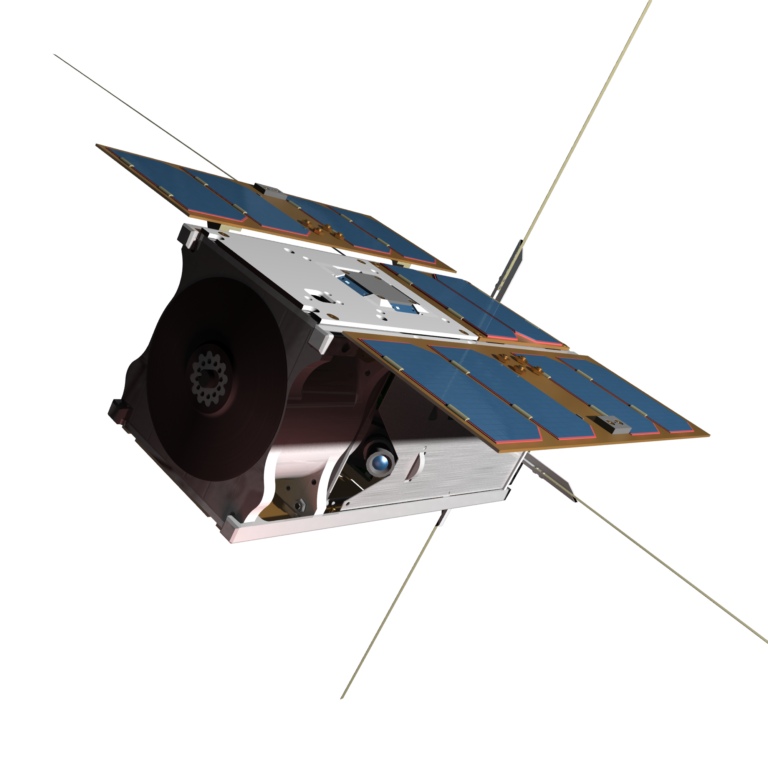
\includegraphics[width=0.38\paperwidth]{img/1/pwsat_solar_panels.png}
    \caption{PW-Sat2 with opened solar panels. Source: \cite{PW_sat2_photo}}
    \label{PW-Sat_solar_panels}
\end{figure}

\subsection{Attitude Determination and Control Subsystem}
Attitude Determination and Control Subsystem (ADCS) is responsible for controlling the satellite orientation. PW-Sat2 implement magnetic control of the orientation using magnetorquers, special type of an electromagnet, designed to interact with Earths' magnetic field. The currents of the magnetorquers are controlled by the subsystem. For PW-Sat2, the only implemented ADCS mode is detumbling - the algorithm to reduce the random tumbling of the satellite to a very low rotational rate (in the order of degrees/second). Therefore, the very slow random tumbling of the satellite is assumed, which forces to use omnidirectional antennas, as the pointing is not possible.

\subsection{Electrical Power System}
Electrical Power System is responsible for power conversion from the solar panels, energy storage in the on-board battery and power distribution to the other subsystems. Electrical power is generated with \si{12} space qualified triple-junction solar cells, resulting in total average power of \SI{1}{\watt} (assuming random tumbling). This energy is harvested by the Electrical Power System and distributed to the other subsystems as shown in the figure \ref{pwsat_eps_distribution}. During the mission, the available average power from the solar panels were assumed: \SI{1.5}{\watt} before sail deployment and \SI{0.75}{\watt} after the sail deployment. The total average power for the communication system was presumed to \SI{0.6}{\watt} average, with peak current consumption of \SI{5}{\watt} during transmission.
\begin{figure}
    \centering
    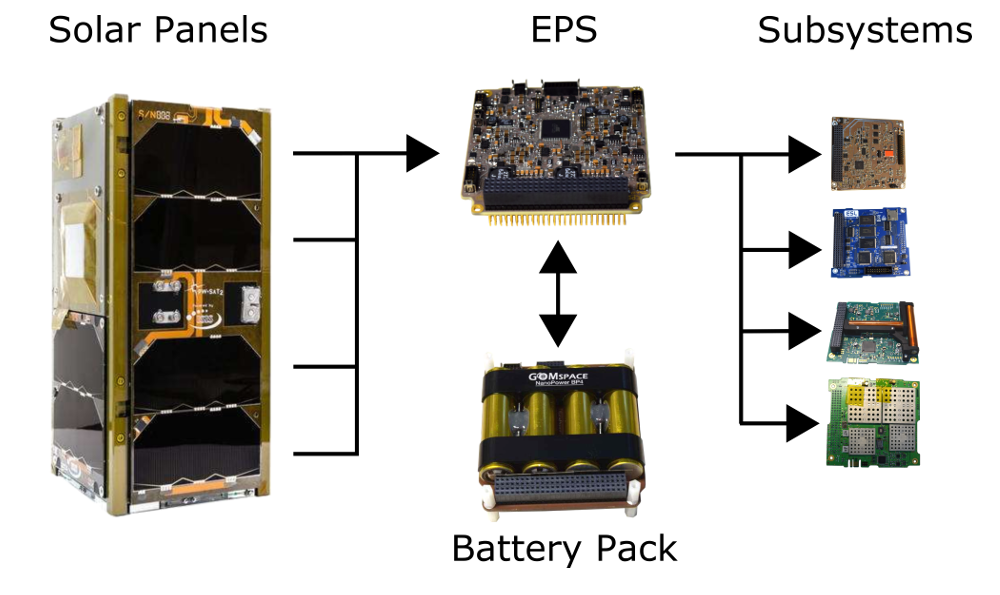
\includegraphics[width=0.7\paperwidth]{img/1/pwsat_eps_distribution.png}
    \caption{PW-Sat2 energy distribution. Source: \cite{PW_sat2_photo}}
    \label{pwsat_eps_distribution}
\end{figure}

\subsection{Mission plan and system lifetime}
PW-Sat2 mission is divided into two phases:
\begin{itemize}
    \item Normal phase - planned to take up to 40 days, before the opening of the deorbit sail. The satellite should perform secondary mission goals during this phase.
    \item Extended phase - activities after the sail deployment. In this phase half of the energy is available for the subsystems. The sail condition and satellite status should be monitored by the operations team up to the moment of satellite deorbitation, by telemetries and photos.
\end{itemize}
